\documentclass[12pt,a4paper]{article}


\usepackage[utf8]{inputenc}
\usepackage[T1]{fontenc}
\usepackage{amsmath}
\usepackage{amsfonts}
\usepackage{amssymb}
\usepackage[francais]{babel}
\usepackage{graphicx}
\usepackage{wrapfig}
\usepackage{hyperref}
\usepackage{cancel}
\usepackage{color}
\usepackage[normalem]{ulem}
\usepackage{soul}
\usepackage[left=2.5cm, right=2.5cm, top=2.5cm, bottom=2.5cm]{geometry}
\usepackage{subfigure}


\newcommand{\com}[1]{{\noindent  \color{red}#1}}   
\newlength{\textlarg}
\newcommand{\barre}[1]{%
   \settowidth{\textlarg}{#1}
   #1\hspace{-\textlarg}\rule[0.5ex]{\textlarg}{0.5pt}}


\author{Baptiste Rouger}
\title{Rapport de stage}
\date{\today}



\begin{document}

	\begin{titlepage}
		
		\begin{center}
			\vfill
			
			{\Huge \textbf{Rapport de stage}}
			
			\vfill
			
			{\LARGE Baptiste \bsc{Rouger}}
			
			~\\L2 BCST
			
			\vfill
			
			{\Huge Analyse de la variation de la taille des plantes lors d'une expérience de sélection divergente pour la date de floraison sur le maïs}
			
			\vfill
			
			{\large\today}
			
			\vfill
			\end{center}
			
			\begin{wrapfigure}[5]{l}[12pt]{5cm}
				
\includegraphics[width=5cm]{logo.jpg}
			\end{wrapfigure} ~\\ %~\\
			UMR de Génétique Quantitative et Evolution - Le Moulon\\
			Ferme du Moulon\\
			91190 Gif-sur-Yvette \\ \\
			
			\begin{figure}[h]
				\centering
				
\includegraphics[width = 4 cm]{inra.jpg}
				
\includegraphics[width = 4 cm]{upsud.jpg}
			\end{figure}
			
			\paragraph*{Directeur de recherche : Olivier \bsc{Martin} \\
			Maître de stage : Christine \bsc{Dillmann}\\
			Enseignant référent : Judith \bsc{Legrand} }
			\vfill
%		\newpage
	\end{titlepage}
	
	\tableofcontents
	\listoffigures
	\newpage
	
	\section*{Glossaire}
	\addcontentsline{toc}{chapter}{Glossaire}
		\begin{description}
			
			\item [Degré-jour :] unité de mesure utilisée pour calculer l'accumulation de chaleur nécessaire à la durée d'un développement biologique comme la croissance d'une plante
			
			\item [Dérive génétique :] réduction du nombre de génotypes différents dans une population de taille finie du fait de l'échantillonnage aléatoire des gamètes ou des individus
			
			\item [Monoïque :] se dit d'une plante dont les fleurs mâles et femelles sont distinctes mais situées sur le même pied
			
			\item [Sélection naturelle :] pression évolutive qui conduit à des changements de la composition génétique d'une population d'une génération à l'autre, en lien avec des différences génétiques des capacités de survie ou de reproduction
			
		
			
		\end{description}
		 
	
	\section{Introduction}
		% faire quelques phrases de présentation ?
		\subsection{Le maïs, une espèce modèle d'intérêt agronomique}
			\subsubsection{Généralités sur le maïs}
				Le maïs (\textit{Zea mays}) est une plante herbacée annuelle appartenant à la famille des \emph{Poacées} (graminées). Par ailleurs, il s'agit d'une plante monoïque.
				Lors de sa domestication (\textit{cf} \ref{histoire_mais}), le maïs a vu certaines de ses caractéristiques changer pour le voir devenir ce qu'il est aujourd'hui. On peut par exemple citer l'absence de dissémination de ses graines, l'augmentation de leur poids et de leur nombre, la synchronisation des dates de floraison mâles et femelles ainsi qu'une dominance apicale entraînant une modification de l'architecture de la plante.
				
				\begin{figure}[h]
					\centering
					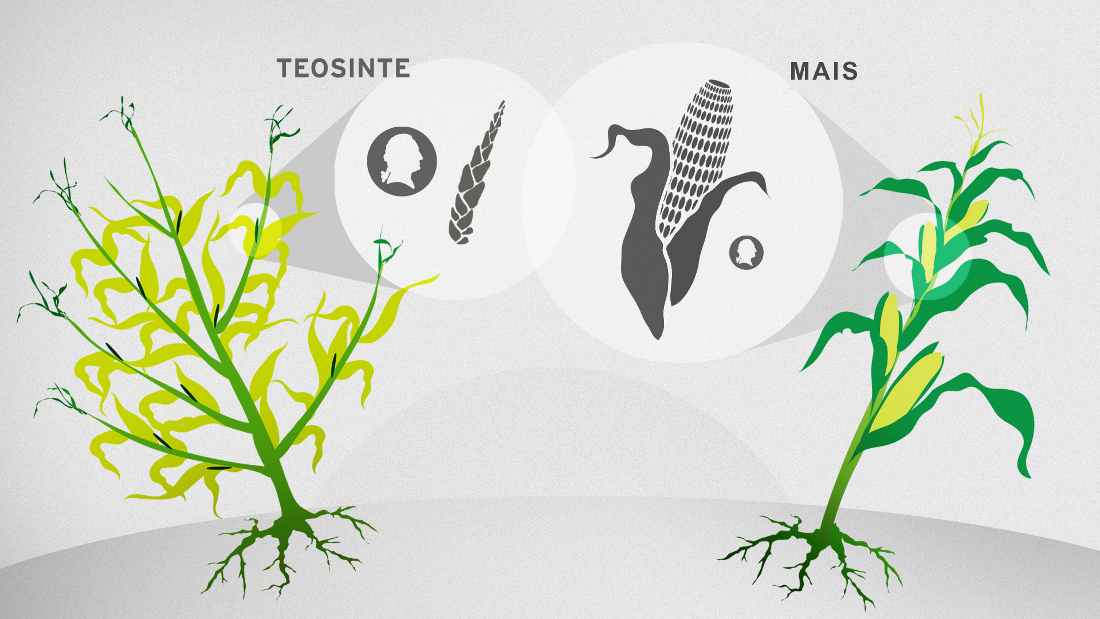
\includegraphics[width=6.6cm]{comparaison.jpg}
					\caption{Comparaison entre téosinte et maïs}
					\label{Comparaison entre téosinte et maïs}
				\end{figure}
				
%				\begin{figure}[!h]
%					\centering
%					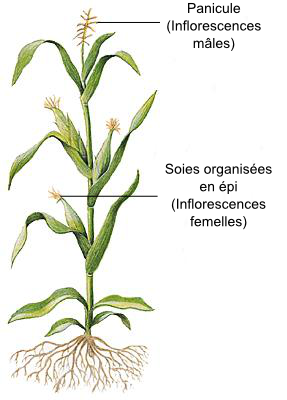
\includegraphics[width=6cm]{monoique.png}
%					\caption{Répartition des organes reproducteurs du maïs}
%					\label{Répartition des organes reproducteurs du maïs}
%				\end{figure}
				\paragraph{Cycle de vie du maïs}
				Le cycle de vie du maïs (\bsc{Figure}~\ref{Cycle de vie du maïs en culture}) commence par la phase de dormance du grain, puis sa germination. Vient ensuite le stade végétatif jeune durant lequel la plante développe ses feuilles juvéniles. Il s'achève par la transition florale qui marque le début du stade végétatif adulte. Celui-ci se termine par la floraison débutant le stade reproducteur. Pour finir, lorsque les graines sont mûres, celles-ci peuvent être récoltées.
				\begin{figure}[h]
					\centering
					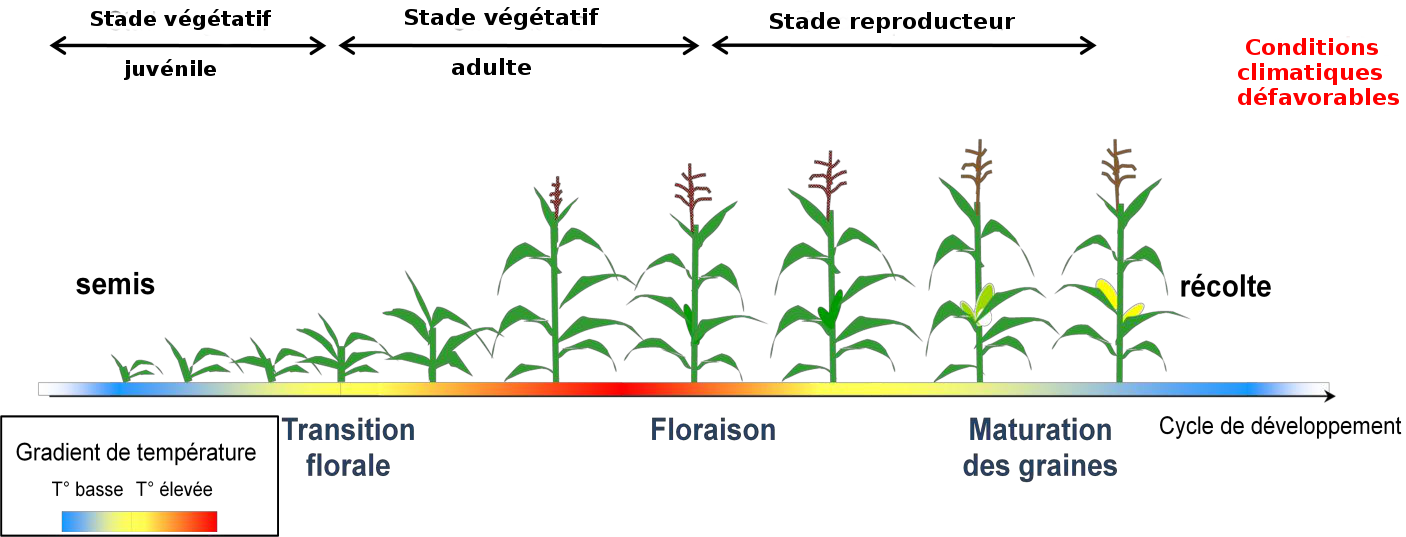
\includegraphics[width=13.7cm]{cycle.png}
					\caption{Cycle de vie du maïs en culture}
					\label{Cycle de vie du maïs en culture}
				\end{figure}
					
			
			\subsubsection{Histoire du maïs}
			\label{histoire_mais}
				Le maïs est une espèce domestiquée depuis environ 9000 ans. Elle est originaire des alentours de Mexico et est issue de la téosinte (\textit{Zea sp}). Elle s'est rapidement propagée à travers le continent américain\cite{tenaillon} en quelques milliers d'années. Cette expansion demanda son adaptation à des climats plus tempérés que son environnement naturel tropical, ce qui fut réalisé en sélectionnant les variétés insensibles à la photopériode, relativement précoces et capables d'effectuer leur cycle de croissance avant l'arrivée des conditions climatiques défavorable (\bsc{Figure}~\ref{Cycle de vie du maïs en culture}). Elle fut découverte et ramenée pour la première fois en Europe par Christophe Colomb lors de sa découverte de l'Amérique. C'est aujourd'hui une des premières céréales cultivées dans le monde.
				
				
		\subsection{Présentation de l'expérience de sélection divergente}
		
			\subsubsection{Généralités}
				
				%parler des degrés jour pour la mesure des durées pour les plantes.
				\paragraph{Des forces évolutives}
				
					Les individus d'une population interagissent de façon dynamique avec leur environnement. Ces interactions conduisent à des changements de composition génétique des populations sous l'effet des pressions évolutives. \textit{Développer...}
					
				\paragraph{L'adaptation}
				
					Il s'agit d'un phénomène résultant des forces évolutives, telle que la sélection. Elle témoigne de la plus grande capacité des individus adaptés à survivre dans leur environnement et à s'y reproduire.
			
			\subsubsection{L'expérience de sélection divergente}
			
				L'expérience de sélection divergente a débuté en 1993. Prenant pour origine deux lignées pures de maïs (F252 et MBS847) à très forte homozygotie, les plants les plus précoces et les plus tardifs pour la date de floraison furent sélectionnés pour le semis chaque année. On obtient ainsi deux populations de maïs pour une même lignée pure, marquants une plus ou moins forte réponse à la sélection selon la variété et la direction de la sélection (\bsc{Figure}~\ref{sélection}).
				\begin{figure}
					\centering
					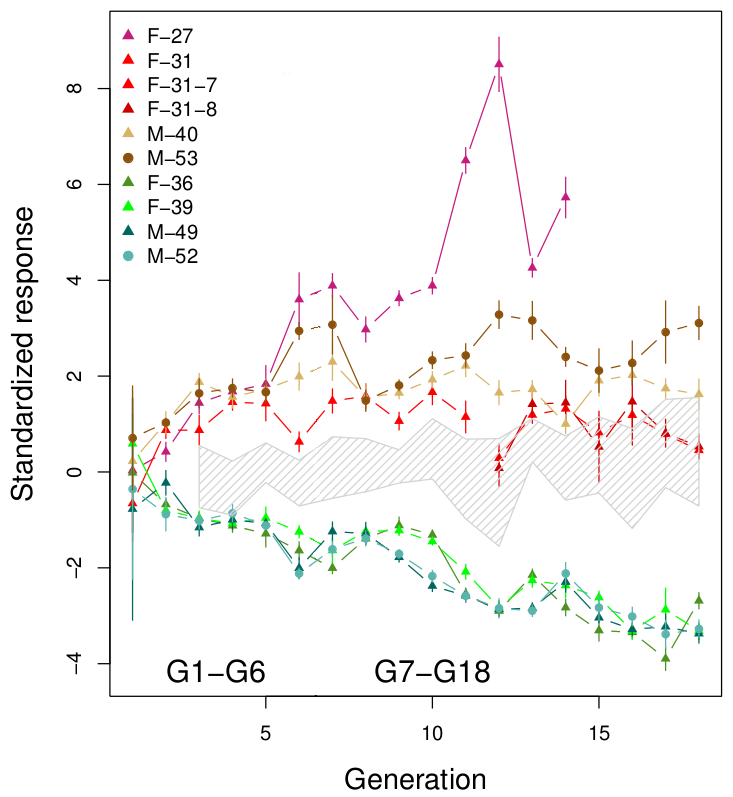
\includegraphics[width =\textwidth]{selection.png}
					\caption{Réponse des deux lignées pures de maïs à la sélection pour la date de floraison}
					\label{sélection}
				\end{figure}
				
				Par ailleurs, la taille des plantes fut aussi mesurée, pour observer si, comment, et combien un caractère n'intervenant pas dans la sélection artificielle d'un individu pouvait être modifié par celle-ci.
			
		\subsection{Objectifs du stage}
		
			Une analyse fine des paramètres de taille pour chaque population de maïs doit être faite pour déterminer dans quelle mesure les plantes voient leur hauteur varier par la sélection faite sur la date de floraison et, le cas échéant, déterminer quelle pourrait être la source de ces variations (mutations, dérive génétique...).
			
	\begin{quotation}
		Après nous êtres intéressés au matériel utilisé lors des vingt années d'expérimentation, nous nous intéresserons au méthodes de traitement des données. Nous analyserons ensuite les résultats et les interpréterons. Enfin, nous conclurons ce sujet.
	\end{quotation}
	
	
	\section{Matériel et méthodes}
		
		\subsection{Le matériel végétal}
			
			L'expérience de sélection divergente (\bsc{Figure}~\ref{selec.div}), débutée en 1993 et toujours en cours, compte 19 générations de maïs. Les lignées de départ utilisées sont deux lignées pures à forte homozygotie : les maïs F252 et MBS847 (notée MBS). On obtient pour chaque lignée deux populations, une tardive et une précoce, sélectionnées pour la date de floraison\footnote{Définie lorsque les fleurs mâles et femelles apparaissent} notée en degrés-jours.
			
			A chaque génération, on réalise pour chaque lignée une autofécondation\footnote{Pour réaliser l'autofécondation, on couvre les fleurs des individus de sachets pour recueillir le pollen et protéger les soies. Après vingt-quatre heures, le sachet contenant le pollen est déposé sur la fleur femelle pour réaliser l'autofécondation.} des dix individus les plus précoces et les plus tardifs. Pour pouvoir retracer le pedigree de chaque individus semé et sélectionné, on réalise des cartes généalogiques (\bsc{Figure}~\ref{carte_gen}) des lignées de maïs. Les individus sélectionnés à la dernière génération sont indiqués en couleur, ainsi que tous leurs descendants. %\cite{goossens93}
			
			\begin{figure}[h]
				
				\begin{minipage}[t]{0.45\textwidth}
					\centering
					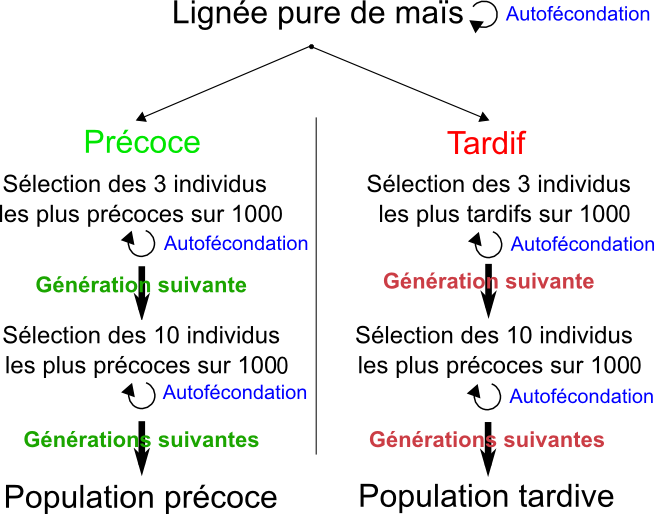
\includegraphics[width=7cm]{selec_div.png} %[width=6.5cm]
					\caption{Principe de l'expérience de sélection divergente}
					\label{selec.div}
				\end{minipage}
				\quad
				\begin{minipage}[t]{0.45\textwidth}
					\centering
					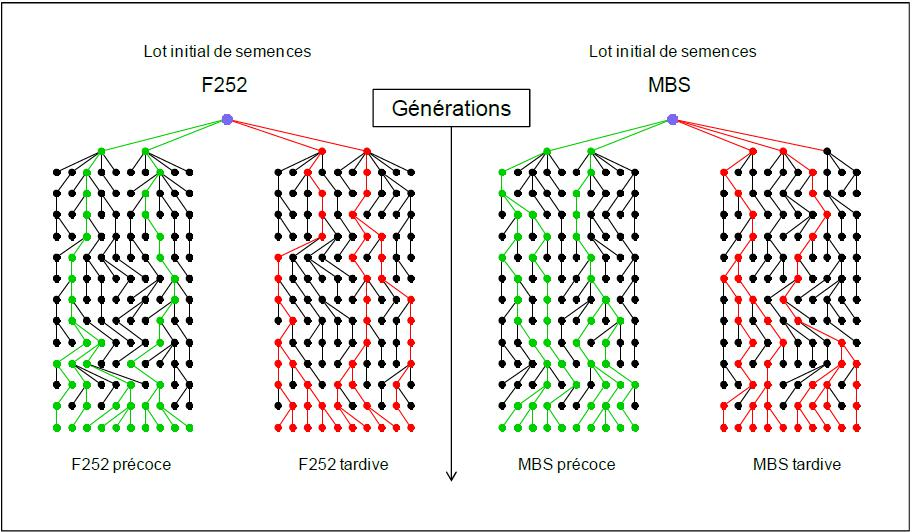
\includegraphics[width=7cm]{carte_gen.jpg} %[width=6.5cm]
					\caption{Généalogie des plantes sélectionnées chez les deux lignées de maïs F252 et MBS pour l'expérience de sélection divergente en 2012}
					\label{carte_gen}
				\end{minipage}
					


				
			\end{figure}
			
		\subsection{Méthodes}
			
			Pour réaliser les analyses nécessaires à la confirmation de nos hypothèses, il faut commencer par formater toutes les données au même format, c'est à dire que chaque plante mesurée sera référencée avec de nombreuses caractéristiques la concernant : l'année, la génération, la lignée (F252 ou MBS), le parent (c'est-à-dire le \og grand-parent \fg de la plante mesurée), le progéniteur (le parent de la plante), la population à laquelle elle appartient (tardive, précoce ou témoin), la famille qui permet de retracer la généalogie, le bloc, la ligne et le numéro de la plante qui permettent de retrouver la position de la plante dans le champs, et bien évidemment la hauteur de la plante.
			
			\subsubsection{Mise en forme des données}
				
				L'ensemble des données que l'on doit rassembler se trouve dans des fichiers de formats différents. Il faut donc les mettre au même format pour commencer à traiter les données. On choisi le format \textbf{CSV} pour des raisons de commodité. Ces fichiers sont ensuite traités par le script\footnote{Tous les scripts sont réalisés dans le langage interprété par le logiciel d'analyses statistiques \textbf{R}. \textit{cf} \bsc{Annexes}~\ref{scripts}} \textit{\ul{tri.R}}. Celui-ci retourne alors un fichier de données formatées par année. Puis le script \textit{\ul{aggregate.R}} permet de rassembler toutes ces données dans un même fichier au format \textbf{CSV}.
			
			\subsubsection{Correction des données}
				
				L'impact de l'année et de l'emplacement dans le champ (appelé \og effet bloc \fg) sur la hauteur des plantes a ensuite été constaté . En effet, il apparaît clair que l'année va jouer un rôle important sur la hauteur de la plante, en fonction de la quantité de précipitations, de la température cumulée, etc. De la même façon, les propriétés du terrain peuvent varier localement, selon par exemple la composition du sol, ce qui va là encore influer sur la hauteur des plantes. Un script\footnote{Il s'agit du script \textit{\ul{DataCorrectv2.R}}} a donc été réalisé pour estimer et corriger les données récoltées.
				
				Ce script réalise une analyse multifactorielle (effet de l'année et \og effet bloc \fg) de la variance de la hauteur. On utilise ensuite les résultats de cette analyse pour corriger dans un premier temps l'\og effet bloc \fg, et dans un second temps l'effet année.
				
		\subsection{Résultats}
			
			\subsubsection{Réponse de la hauteur des plantes à la sélection pour la date de floraison}
			
				Grâce aux deux graphiques suivants ( \bsc{Figure}~\ref{hauteursf252}(c) et \bsc{Figure}~\ref{hauteursmbs}(c)), on peut conclure que les données peuvent être corrigées, puisque les témoins ont tous deux une droite de régression dont le coefficient directeur est de 0.\\
				
				Par ailleurs, on constate que la variation de taille, bien que significative, est relativement faible au fil des années ( < 1 cm/an) à partir de 1998.\\
				Cela semble indiquer qu'une réponse à la sélection très rapide a eu lieu, laissant ensuite la place à une réponse beaucoup plus faible, voire insignifiante.\\
	
				On observe également\footnote{\bsc{Figure}~\ref{hauteursf252} et \bsc{Figure}~\ref{hauteursmbs}} des tendances à la hausse pour les populations tardives (0.53 cm/an et 0.21 cm/an respectivement pour F252 et MBS) et une tendance à la baisse pour les populations précoces de MBS (-0.64 cm/an). Les populations précoce de F252 semblent cependant augmenter de taille, bien que très faiblement (0.03 cm/an).\\
				
				\begin{figure} %[h]
					\begin{minipage}[t]{0.32\textwidth}
						\subfigure[Population précoce]{
							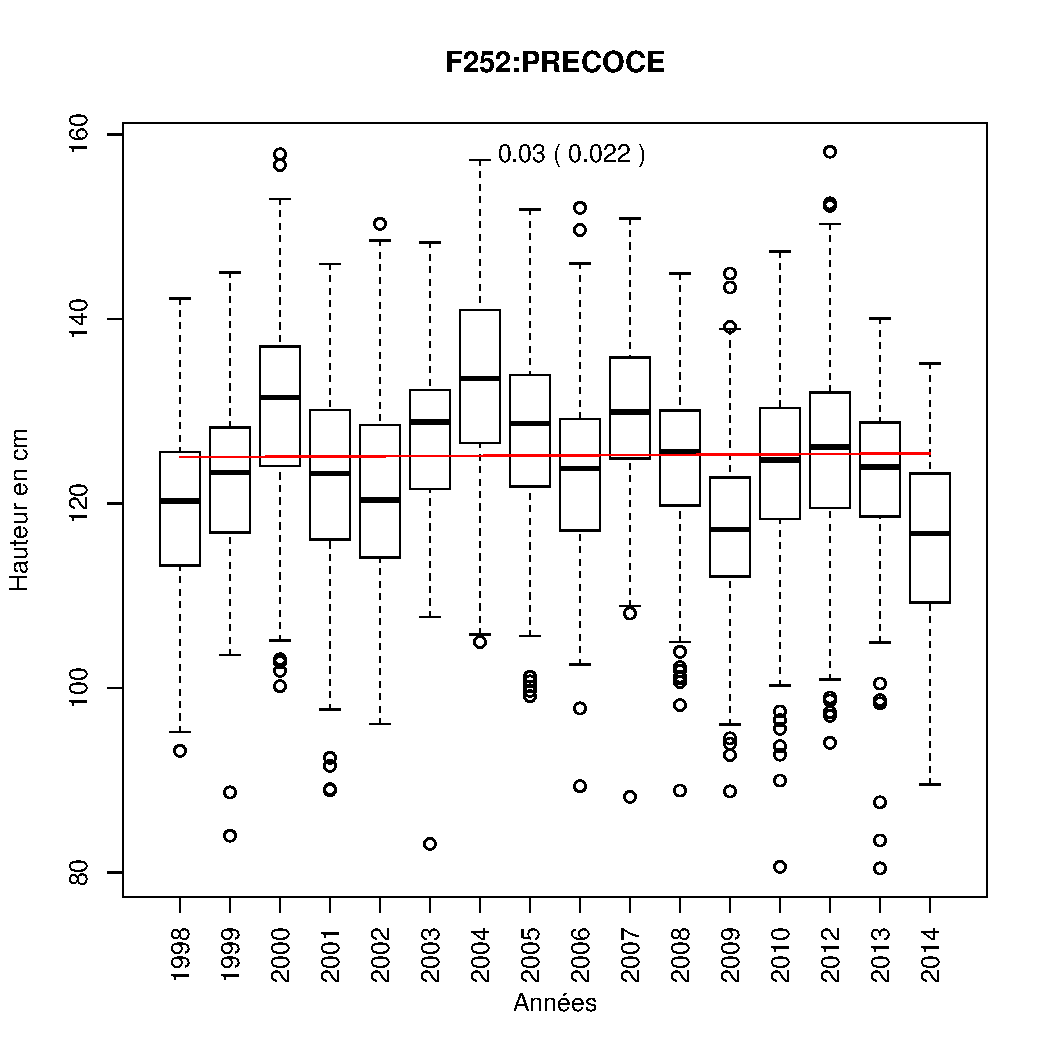
\includegraphics[width=4.5cm]{plot_haut_pop_F252_PRECOCE.pdf}
						}
					\end{minipage}
					\begin{minipage}[t]{0.32\textwidth}
						\subfigure[Population précoce]{
							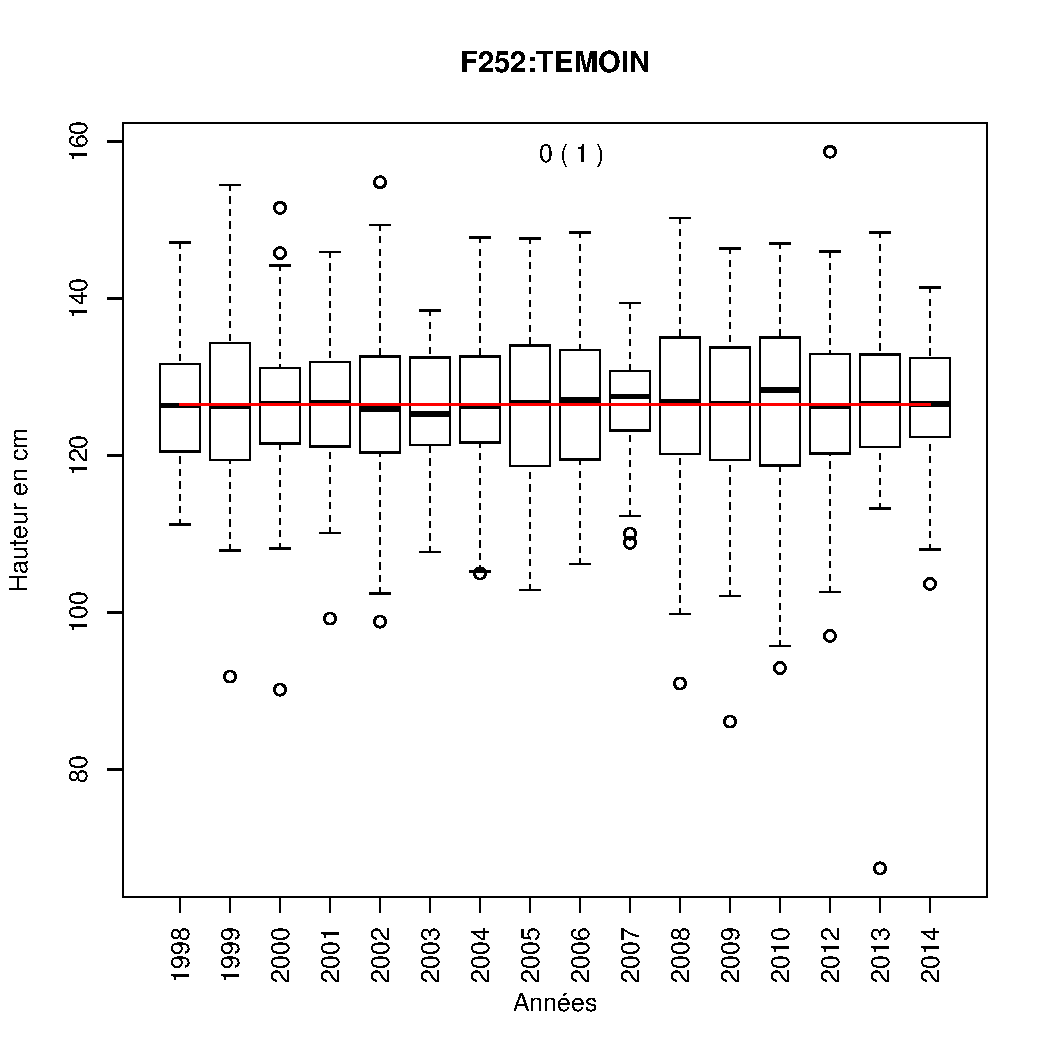
\includegraphics[width=4.5cm]{plot_haut_pop_F252_TEMOIN.pdf}
						}
					\end{minipage}
					\begin{minipage}[t]{0.32\textwidth}
						\subfigure[Population précoce]{
							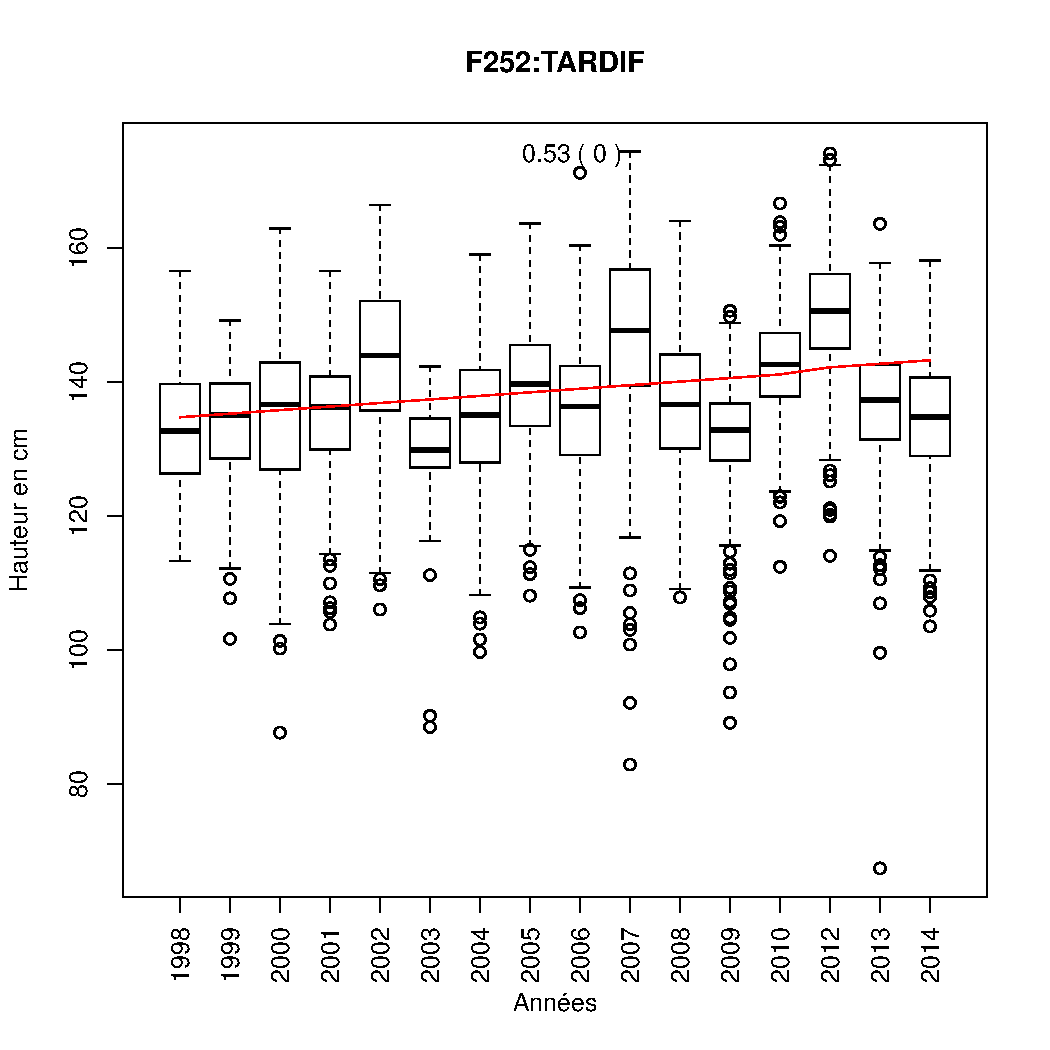
\includegraphics[width=4.5cm]{plot_haut_pop_F252_TARDIF.pdf}
						}
					\end{minipage}
					\caption{Représentation des hauteurs des plantes de la lignée F252 \label{hauteursf252}}
				\end{figure}
				\quad
				\begin{figure} %[h]
					\begin{minipage}[t]{0.32\textwidth}
						\subfigure[Population précoce]{
							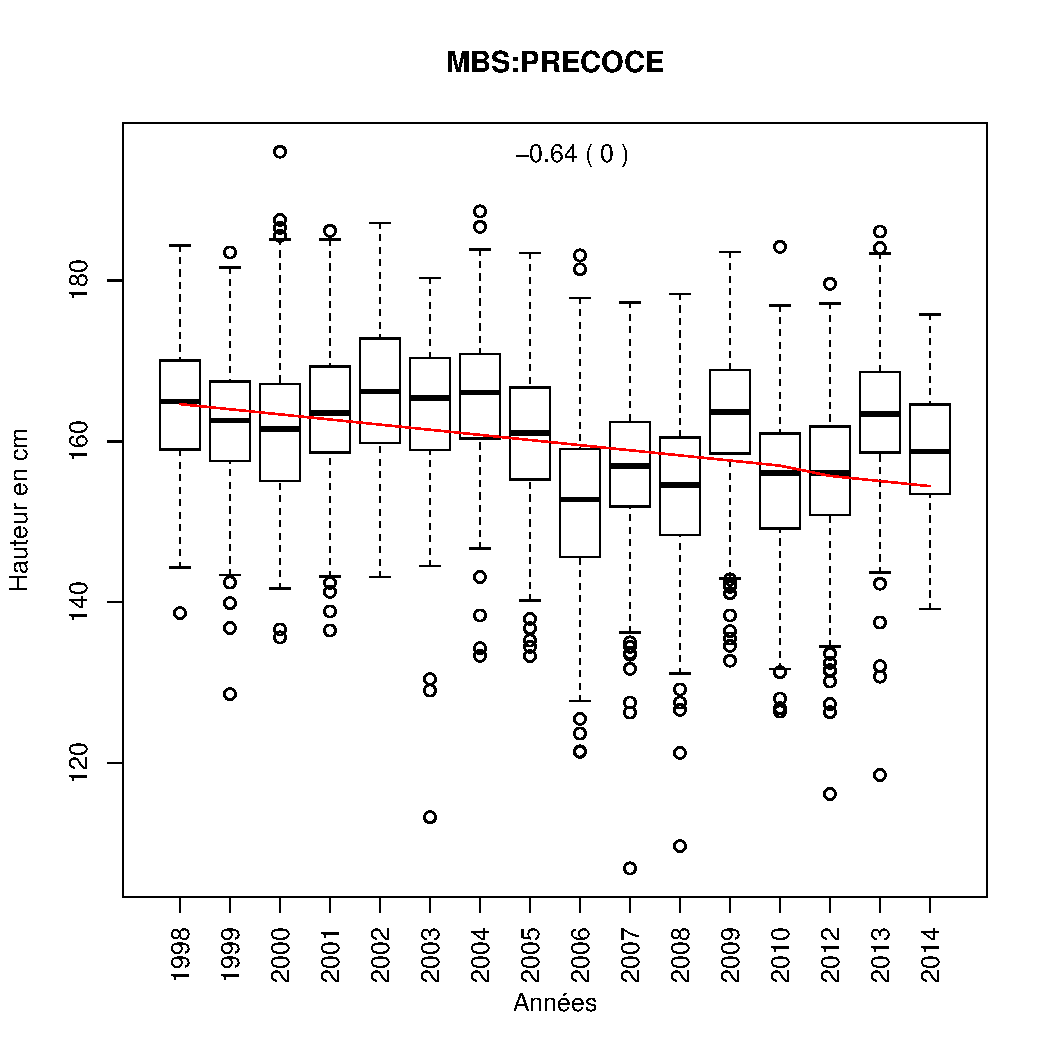
\includegraphics[width=4.5cm]{plot_haut_pop_MBS_PRECOCE.pdf}
						}
					\end{minipage}
					\begin{minipage}[t]{0.32\textwidth}
						\subfigure[Population précoce]{
							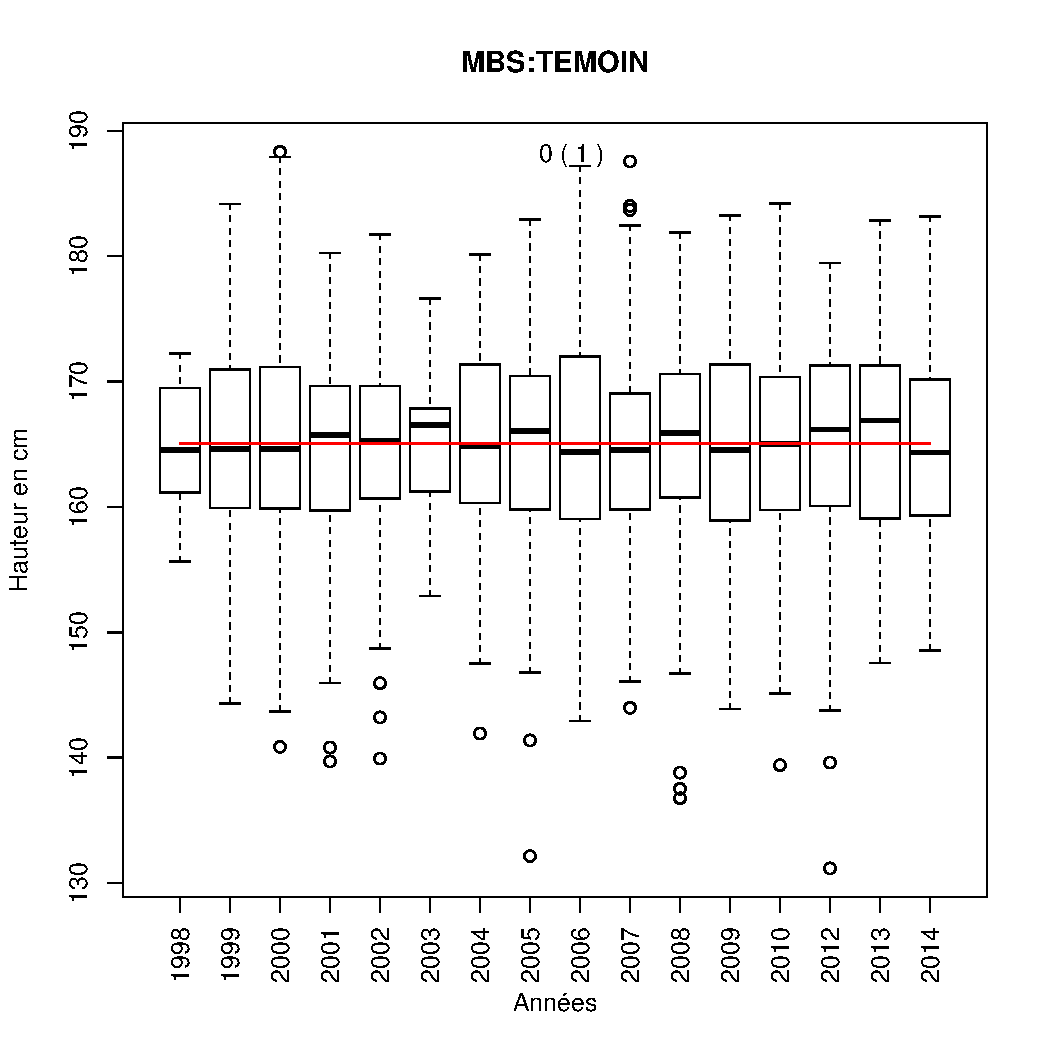
\includegraphics[width=4.5cm]{plot_haut_pop_MBS_TEMOIN.pdf}
						}
					\end{minipage}
					\begin{minipage}[t]{0.32\textwidth}
						\subfigure[Population précoce]{
							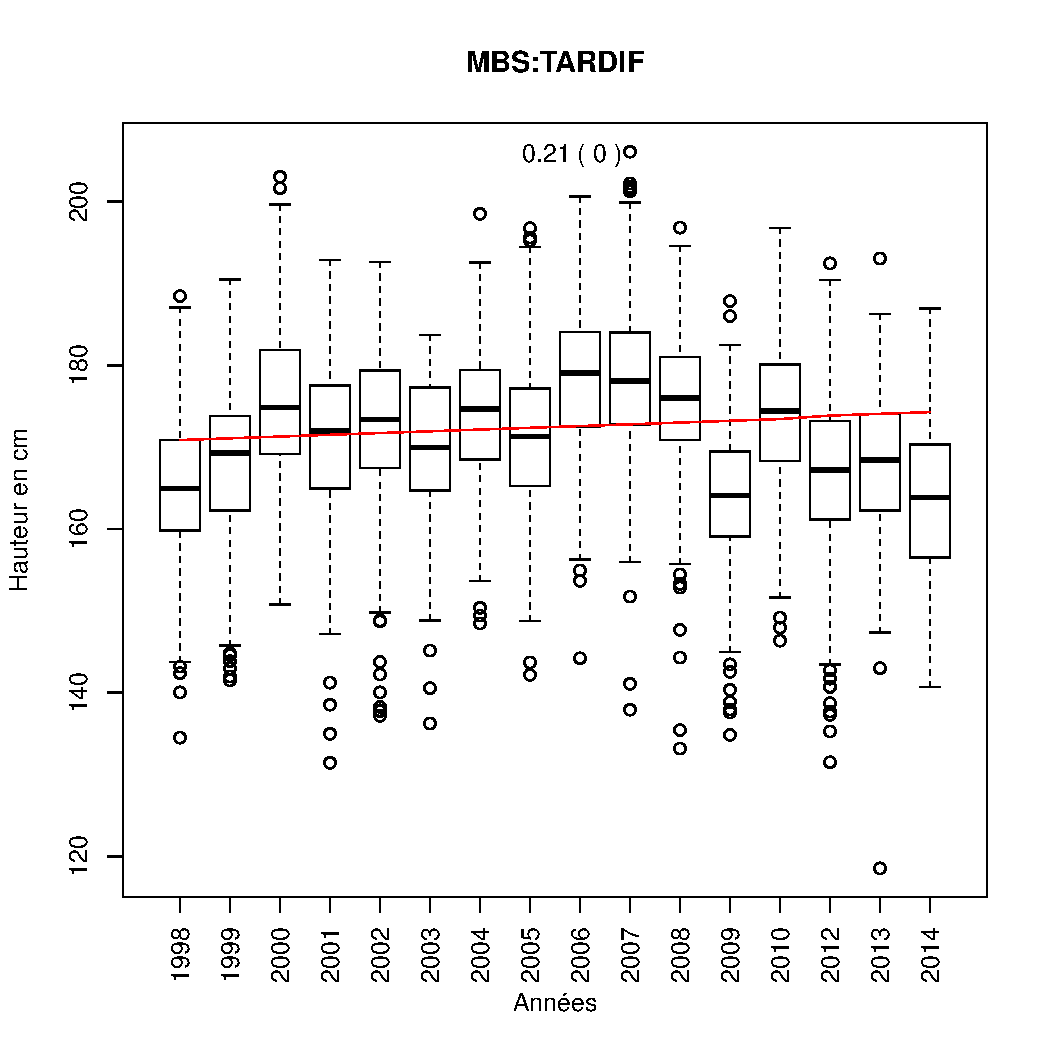
\includegraphics[width=4.5cm]{plot_haut_pop_MBS_TARDIF.pdf}
						}
					\end{minipage}
					\caption{Représentation des hauteurs des plantes de la lignée MBS \label{hauteursmbs}}
				\end{figure}

			\subsubsection{Corrélation entre hauteur et date de floraison}
				
				\paragraph{Corrélation par famille et par année}
				Il a également été testée si il y avait bien une corrélation entre la hauteur des plantes et la date de floraison (\bsc{Figure}~\ref{correlation}). Pour cela, on représente pour chaque famille et chaque année la hauteur moyenne des plantes en fonction de leur date moyenne de floraison.\\
				On peut voir que les points semblent globalement être répartis autour d'une droite, ce qui confirme la corrélation entre hauteur et date de floraison. 
				
				On peut également observer une scission entre les populations précoces et tardives des lignées (respectivement dans les couleurs bleu/vert et rouge en \bsc{Figure}~\ref{correlation}).
				
				
				
				
				
				On remarque cependant que, malgré que l'ensemble des points confirme la corrélation, certaines familles ne semblent pas suivre cette dernière. Par exemple, la famille F-39 ( \bsc{Figure}~\ref{correl.fam}) ne montre plus de corrélation, tandis que pour M-49 ( \bsc{Figure}~\ref{correl.fam}), elle apparaît conservée. 
				
				\begin{figure}[!h]
						\subfigure{
							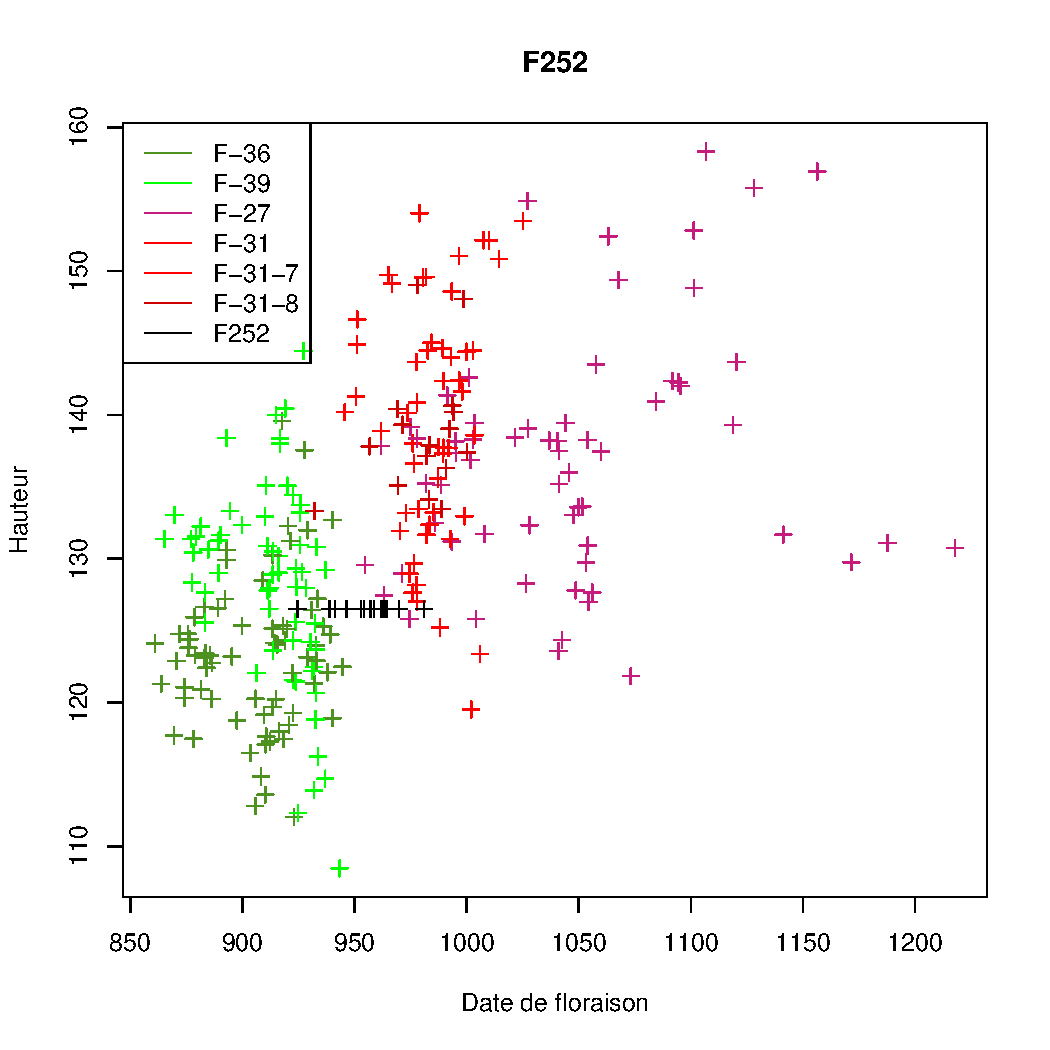
\includegraphics[width=0.45\textwidth]{plot_haut-flo_F252.pdf}
						}
						\subfigure{
							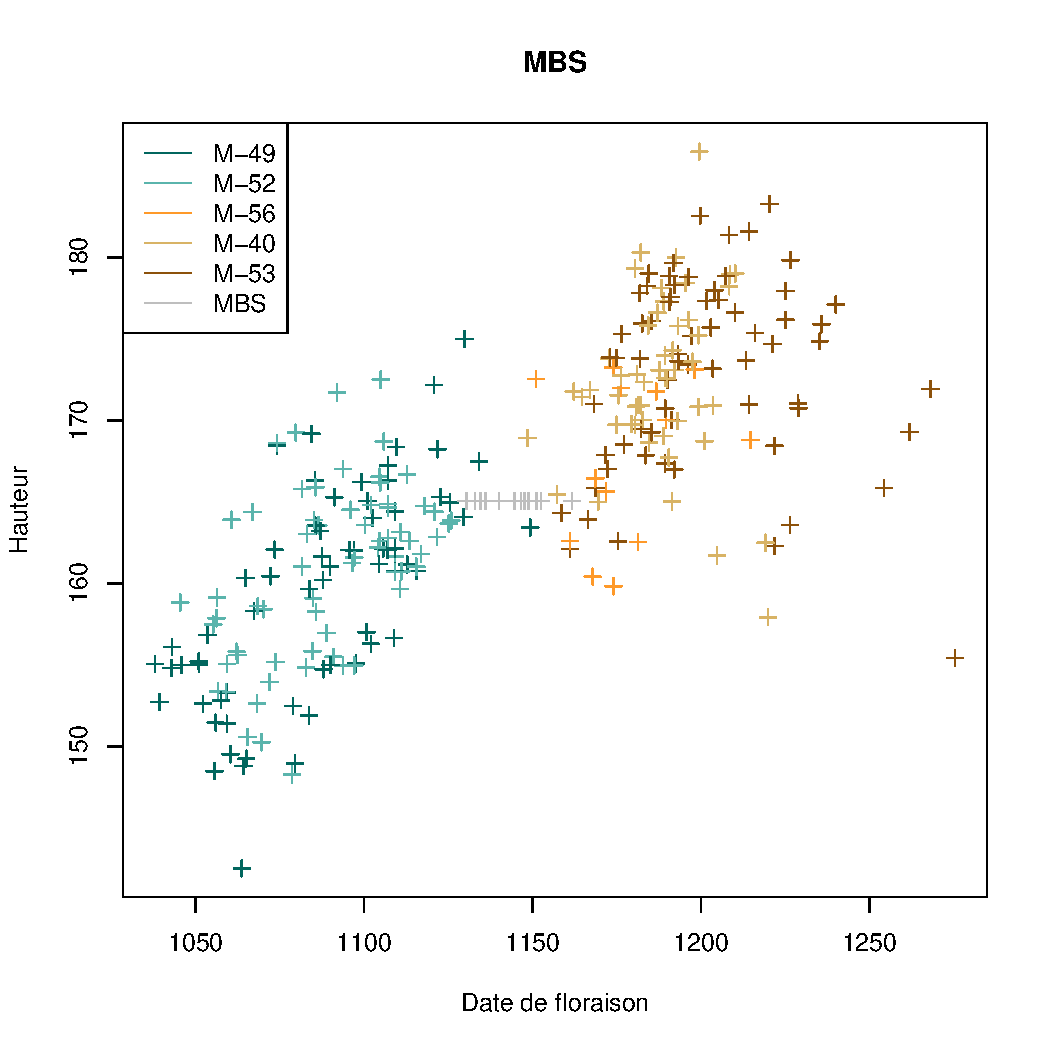
\includegraphics[width=0.45\textwidth]{plot_haut-flo_MBS.pdf}
						}
					\caption{Représentation de la relation entre hauteur et date de floraison \label{correlation}}
					Chaque point d'une couleur représente la moyenne de la hauteur des progéniteurs d'une famille pour une année (couleurs dans la figure) en fonction de la date moyenne de floraison de ces mêmes plantes. A gauche, la lignée F252 et à droite la lignée MBS.
				\end{figure}
				
				\begin{figure}[!h]
					\subfigure{
						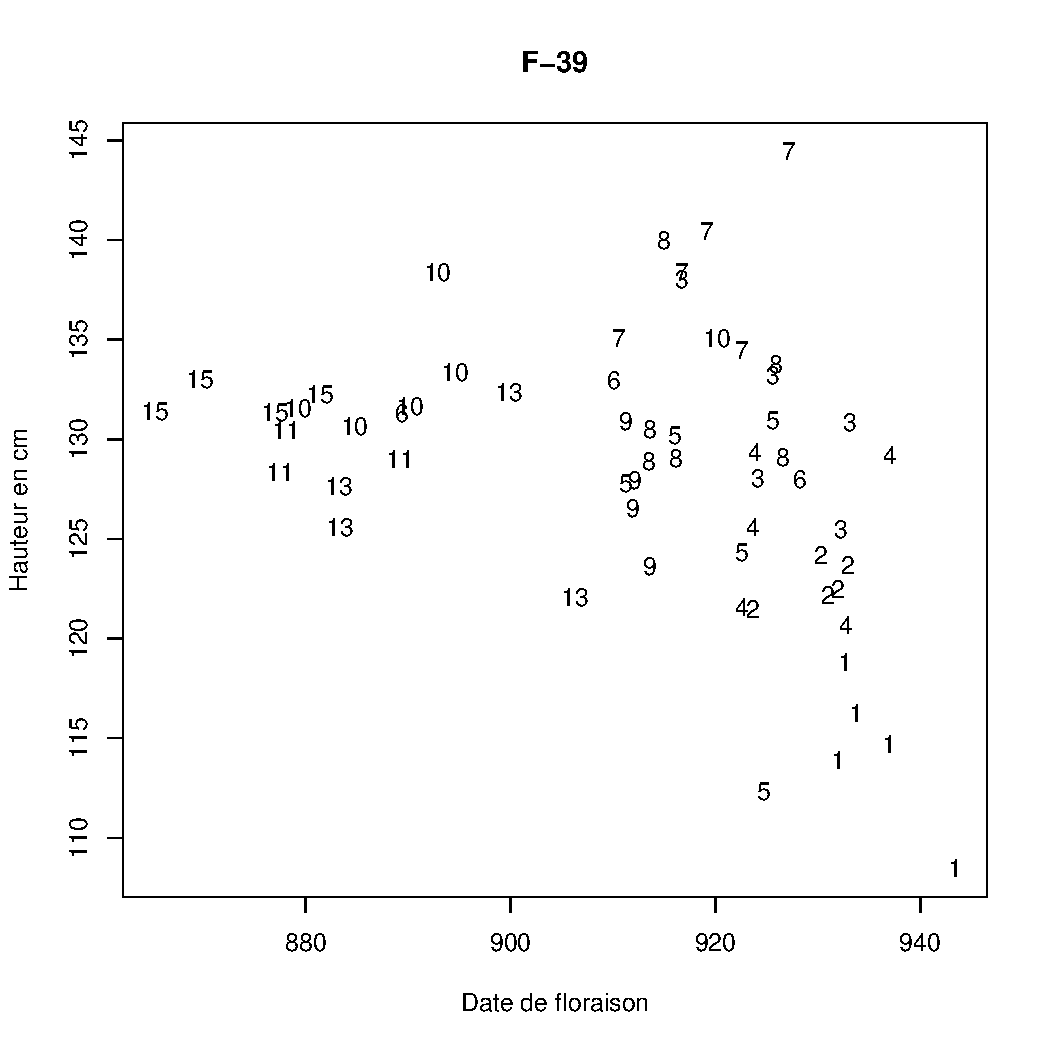
\includegraphics[width=0.45\textwidth]{plot_haut-flo_f39.pdf}
					}
					\subfigure{
						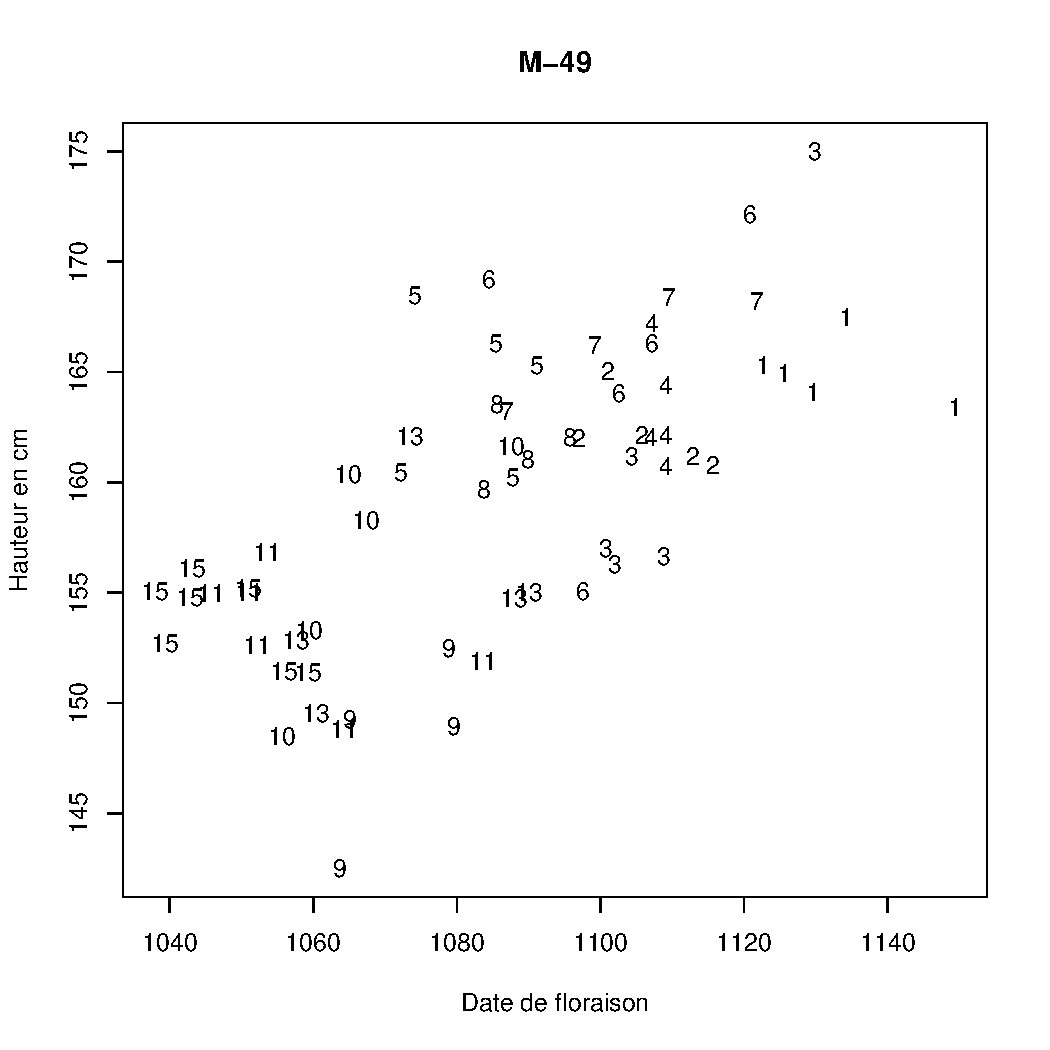
\includegraphics[width=0.45\textwidth]{plot_haut-flo_m49.pdf}
					}
					\caption{Représentation séparée de la corrélation entre hauteur et date de floraison pour deux familles \label{correl.fam}}
					Chaque point représente la moyenne de la hauteur des progéniteurs de la famille (F-39 à gauche et M-49 à droite) pour une année en fonction de la date moyenne de floraison de ces mêmes plantes.
				\end{figure}
				
			\paragraph{Corrélation par individu pour 2013 et 2014}
				
				On peut voir que ça fait des choses bizarres...
				
				\begin{figure}[h]
					\centering
					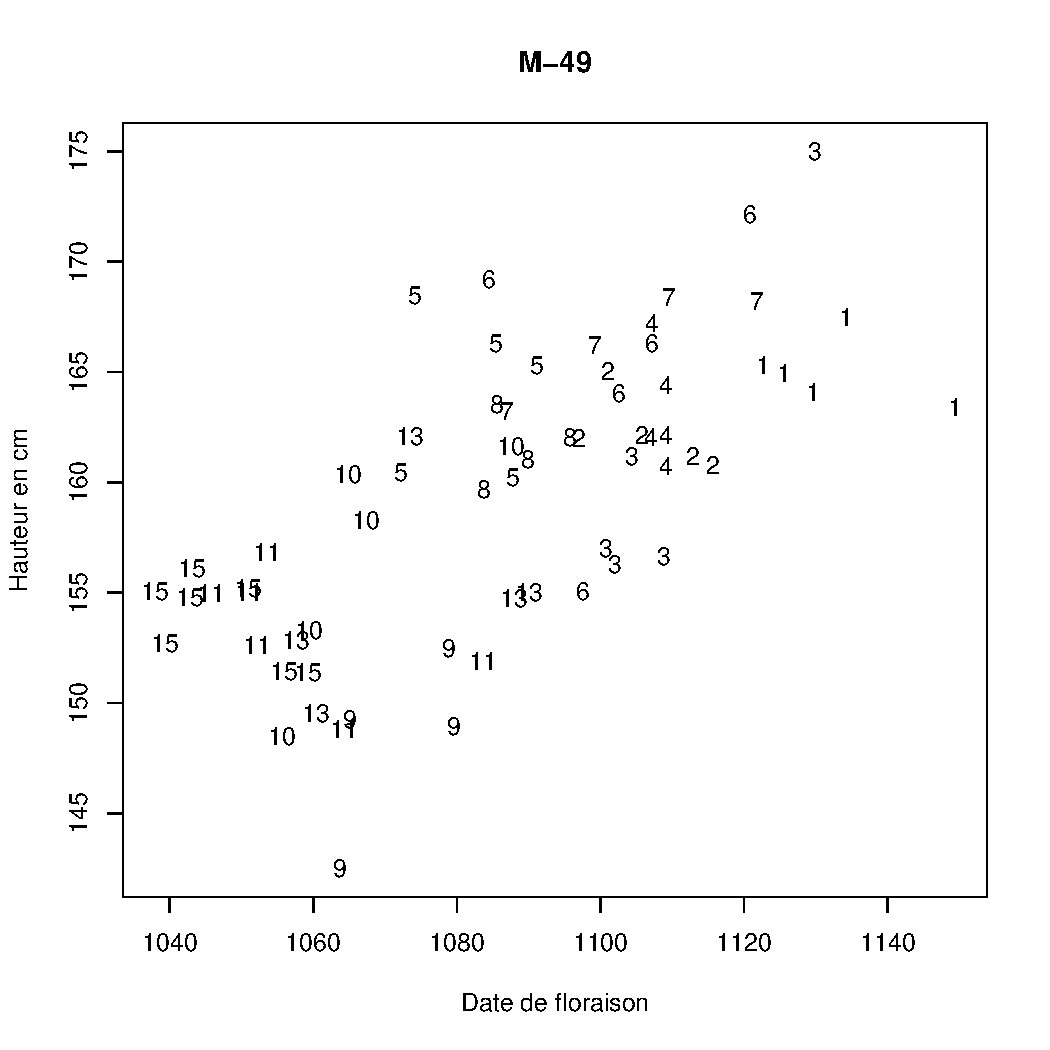
\includegraphics[width=0.45\textwidth]{plot_haut-flo_m49.pdf}
					\caption{Répresentation de la corrélation entre hauteur et date de floraison par individus en 2013 et 2014 \label{correl.ind}}
				\end{figure}
			
				
	\bibliographystyle{plain}
	\bibliography{rapport}
	
	\appendix
	
	\section{Codes sources}
	\label{scripts}
	Les codes sources utilisés pendant ce stage sont disponibles sur Github à l'adresse suivante : \url{https://github.com/rougerbaptiste/stageL2}.\\~\\
	Voici la fonction de chacun de ces codes :
	\begin{description}
		\item [aggregate.R :] Ce script a pour fonction de rassembler les données contenues dans les fichiers de hauteurs de chaque année pour les rassembler dans un unique fichier.
		\item [Datacorrectv2.R :] Ce script corrige les données des années et affiche un graphe (\textit{Référence}) résumant les données.
		\item [RprFam.R :] Ce script a pour fonction de représenter les données de hauteurs obtenues pour chaque famille (hauteur absolue et hauteur relative au témoin) et de créer un fichier .pdf contenant les deux graphes.
		\item [RprPop.R :] Ce script a pour fonction de représenter les données de hauteurs obtenues pour chaque population (hauteur absolue et hauteur relative au témoin) et de créer un fichier .pdf contenant les deux graphes.
		\item [tri.R :] Ce script a pour fonction de récupérer toutes les données brutes de hauteurs, de les mettre sous une forme standard et de créer un fichier contenant les données de hauteur par année.
		
	\end{description}
\end{document}
